\PassOptionsToPackage{unicode=true}{hyperref} % options for packages loaded elsewhere
\PassOptionsToPackage{hyphens}{url}
%
\documentclass[
  ignorenonframetext,
]{beamer}
\usepackage{pgfpages}
\setbeamertemplate{caption}[numbered]
\setbeamertemplate{caption label separator}{: }
\setbeamercolor{caption name}{fg=normal text.fg}
\beamertemplatenavigationsymbolsempty
% Prevent slide breaks in the middle of a paragraph:
\widowpenalties 1 10000
\raggedbottom
\setbeamertemplate{part page}{
  \centering
  \begin{beamercolorbox}[sep=16pt,center]{part title}
    \usebeamerfont{part title}\insertpart\par
  \end{beamercolorbox}
}
\setbeamertemplate{section page}{
  \centering
  \begin{beamercolorbox}[sep=12pt,center]{part title}
    \usebeamerfont{section title}\insertsection\par
  \end{beamercolorbox}
}
\setbeamertemplate{subsection page}{
  \centering
  \begin{beamercolorbox}[sep=8pt,center]{part title}
    \usebeamerfont{subsection title}\insertsubsection\par
  \end{beamercolorbox}
}
\AtBeginPart{
  \frame{\partpage}
}
\AtBeginSection{
  \ifbibliography
  \else
    \frame{\sectionpage}
  \fi
}
\AtBeginSubsection{
  \frame{\subsectionpage}
}
\usepackage{lmodern}
\usepackage{amssymb,amsmath}
\usepackage{ifxetex,ifluatex}
\ifnum 0\ifxetex 1\fi\ifluatex 1\fi=0 % if pdftex
  \usepackage[T1]{fontenc}
  \usepackage[utf8]{inputenc}
  \usepackage{textcomp} % provides euro and other symbols
\else % if luatex or xelatex
  \usepackage{unicode-math}
  \defaultfontfeatures{Scale=MatchLowercase}
  \defaultfontfeatures[\rmfamily]{Ligatures=TeX,Scale=1}
\fi
\usetheme[]{CambridgeUS}
\usecolortheme{dove}
\usefonttheme{professionalfonts}
% use upquote if available, for straight quotes in verbatim environments
\IfFileExists{upquote.sty}{\usepackage{upquote}}{}
\IfFileExists{microtype.sty}{% use microtype if available
  \usepackage[]{microtype}
  \UseMicrotypeSet[protrusion]{basicmath} % disable protrusion for tt fonts
}{}
\makeatletter
\@ifundefined{KOMAClassName}{% if non-KOMA class
  \IfFileExists{parskip.sty}{%
    \usepackage{parskip}
  }{% else
    \setlength{\parindent}{0pt}
    \setlength{\parskip}{6pt plus 2pt minus 1pt}}
}{% if KOMA class
  \KOMAoptions{parskip=half}}
\makeatother
\usepackage{xcolor}
\IfFileExists{xurl.sty}{\usepackage{xurl}}{} % add URL line breaks if available
\IfFileExists{bookmark.sty}{\usepackage{bookmark}}{\usepackage{hyperref}}
\hypersetup{
  pdftitle={Anotation Redundancy},
  pdfauthor={Jun Kang},
  pdfborder={0 0 0},
  breaklinks=true}
\urlstyle{same}  % don't use monospace font for urls
\newif\ifbibliography
\usepackage{graphicx,grffile}
\makeatletter
\def\maxwidth{\ifdim\Gin@nat@width>\linewidth\linewidth\else\Gin@nat@width\fi}
\def\maxheight{\ifdim\Gin@nat@height>\textheight\textheight\else\Gin@nat@height\fi}
\makeatother
% Scale images if necessary, so that they will not overflow the page
% margins by default, and it is still possible to overwrite the defaults
% using explicit options in \includegraphics[width, height, ...]{}
\setkeys{Gin}{width=\maxwidth,height=\maxheight,keepaspectratio}
\setlength{\emergencystretch}{3em}  % prevent overfull lines
\providecommand{\tightlist}{%
  \setlength{\itemsep}{0pt}\setlength{\parskip}{0pt}}
\setcounter{secnumdepth}{-2}

% set default figure placement to htbp
\makeatletter
\def\fps@figure{htbp}
\makeatother

\usepackage{graphicx}
\usepackage{tikzpagenodes}
\usetikzlibrary{calc}
\usepackage{caption}
\usepackage{booktabs}
\usepackage{longtable}
\usepackage{array}
\usepackage{multirow}
\usepackage{multicol}
\usepackage{wrapfig}
\usepackage{float}
\usepackage{colortbl}
\usepackage{pdflscape}
\usepackage{tabu}
\usepackage{threeparttable}

\title{Anotation Redundancy}
\author{Jun Kang}
\date{2019-11-01}

\begin{document}
\frame{\titlepage}

\begin{frame}{Annotation redundancy}
\protect\hypertarget{annotation-redundancy}{}

\begin{itemize}
\tightlist
\item
  Exact variants (indication for targeted therapy)\\
\item
  \textbf{Many annotations} for a \textbf{same variant}
\end{itemize}

\end{frame}

\begin{frame}{Case 1}
\protect\hypertarget{case-1}{}

5.3cm, central mass in LUL, obstructing LUL bronchus Suspicious invasion
of left upper pulmonary artery

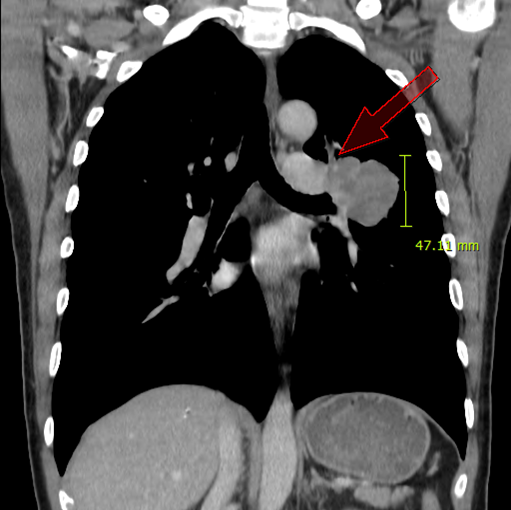
\includegraphics[width=\textwidth,height=4.16667in]{assets/img/chest_ct.png}

\end{frame}

\begin{frame}

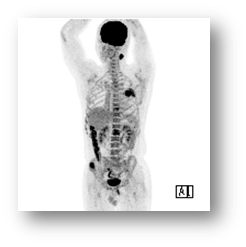
\includegraphics[width=\textwidth,height=4.16667in]{assets/img/bone_scan.png}

\end{frame}

\begin{frame}{Pathology}
\protect\hypertarget{pathology}{}

\begin{itemize}
\tightlist
\item
  Lymph node, level II, left, needle biopsy;
\item
  \textbf{Adenocarcinoma, solid type} \textbf{,} \textbf{metastatic}
\item
  PD-L1: 22C3(0\%), SP142(0\%)
\end{itemize}

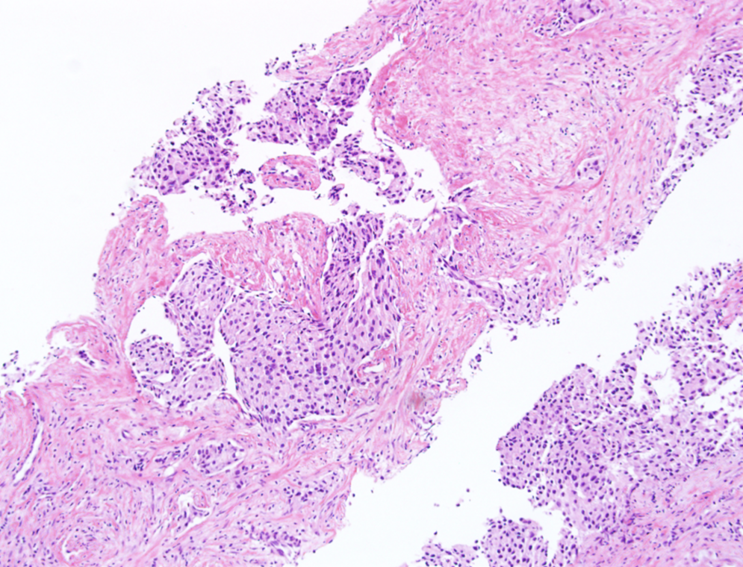
\includegraphics[width=\textwidth,height=4.16667in]{assets/img/biopsy.png}

\end{frame}

\begin{frame}{TTF-1}
\protect\hypertarget{ttf-1}{}

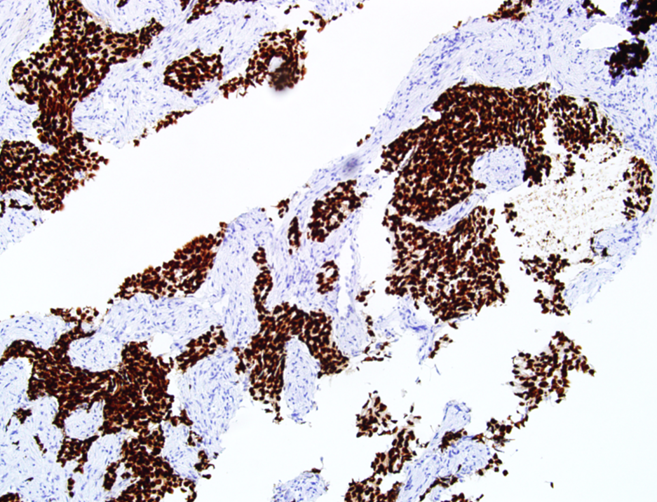
\includegraphics[width=\textwidth,height=4.16667in]{assets/img/immuno.png}

\end{frame}

\begin{frame}{Molecular}
\protect\hypertarget{molecular}{}

\begin{itemize}
\tightlist
\item
  \textbf{EGFR} \textbf{PNAClamp} : negative
\item
  \textbf{FISH} : ALK(-), ROS1(-), RET(-)
\end{itemize}

\end{frame}

\begin{frame}{NGS (Ion Torrent)}
\protect\hypertarget{ngs-ion-torrent}{}

\begin{itemize}
\tightlist
\item
  ERBB2 exon20 insertion\\
\item
  Afatinib: irreversible EGFR TKI
\end{itemize}

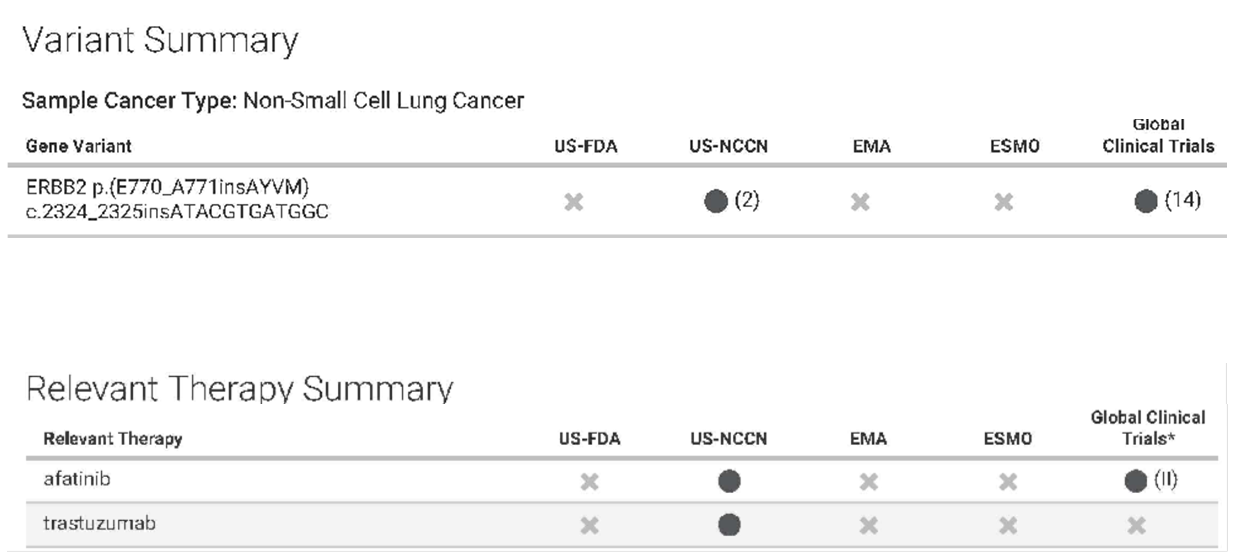
\includegraphics{assets/img/OCR.png}

\end{frame}

\begin{frame}{Ion Reporter, COSMIC, VEP (Variant Effect Predictor,
Ensembl)\textsuperscript{1}}
\protect\hypertarget{ion-reporter-cosmic-vep-variant-effect-predictor-ensembl--__what_}{}

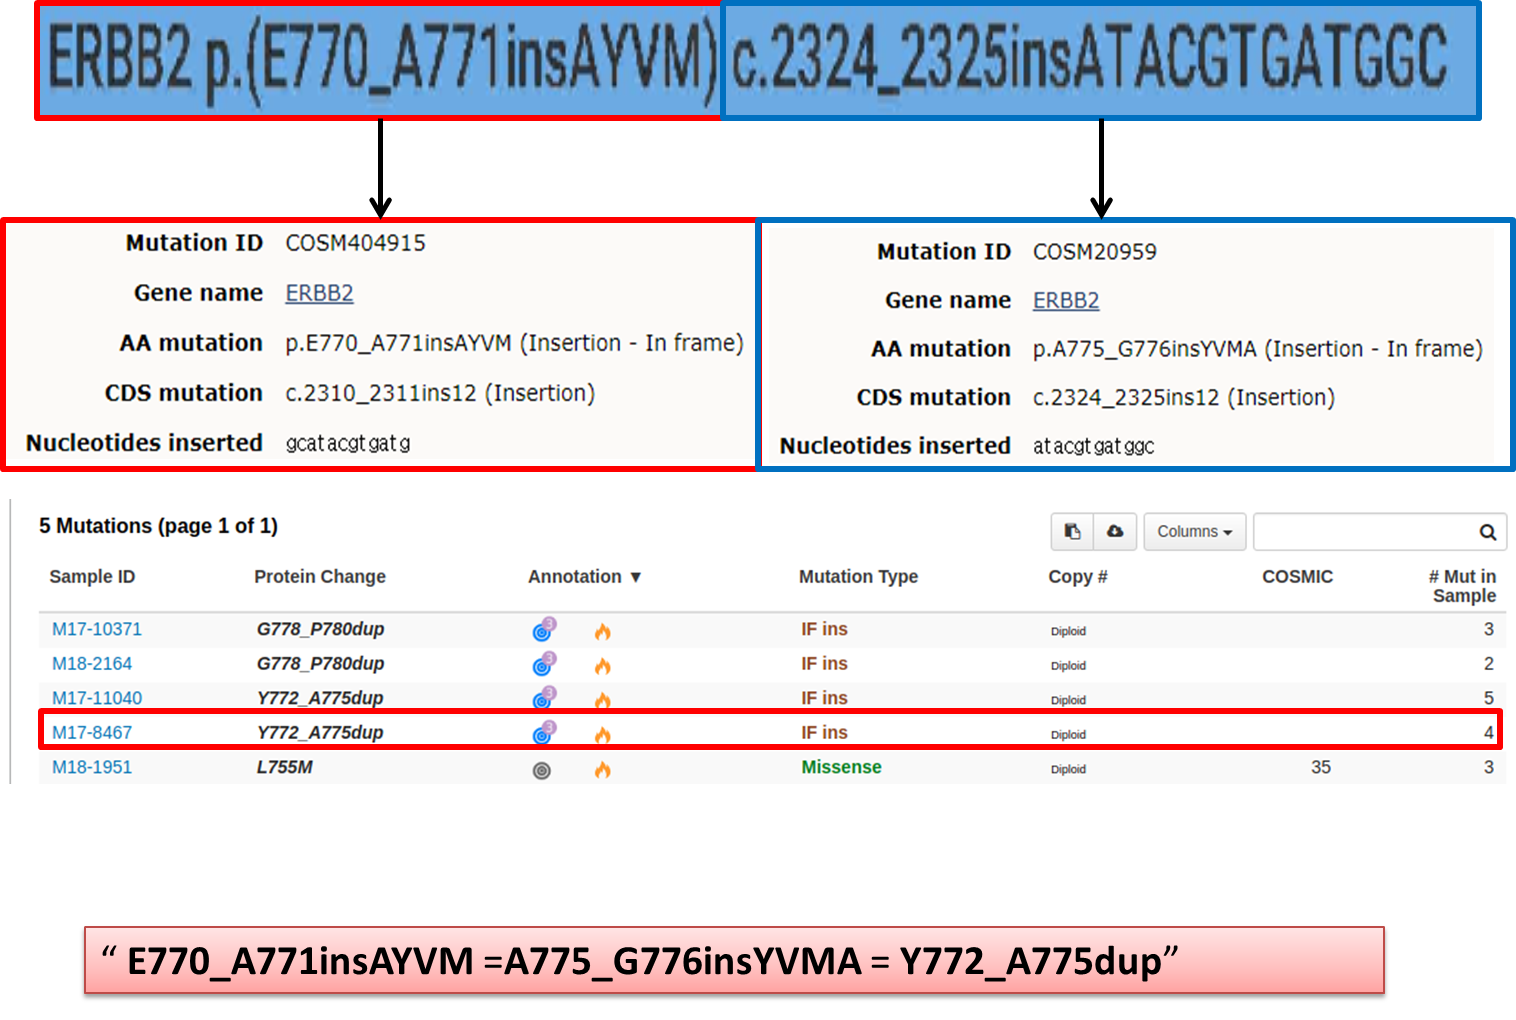
\includegraphics{assets/img/erbb2_cmc.png}

\end{frame}

\begin{frame}{Redundant annotations for ERBB2 insertion mutation}
\protect\hypertarget{redundant-annotations-for-erbb2-insertion-mutation}{}

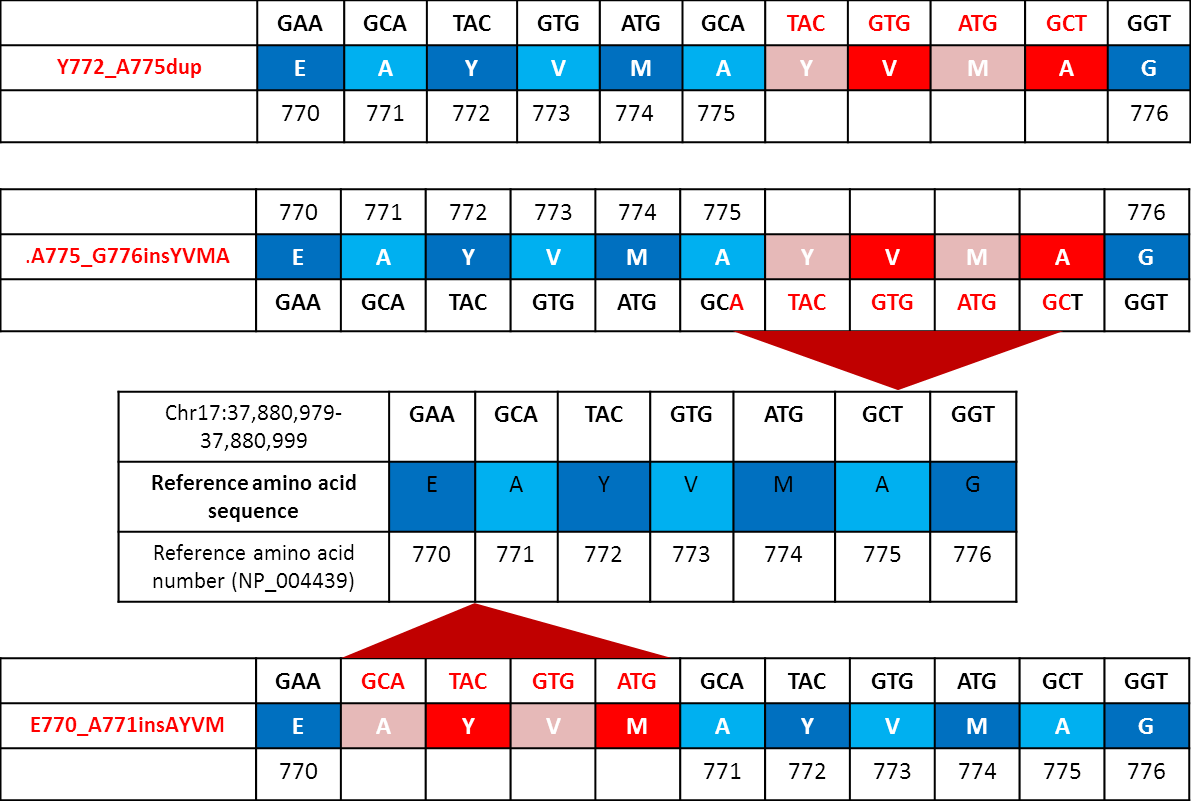
\includegraphics[width=\textwidth,height=2.08333in]{assets/img/insertion.png}

\end{frame}

\begin{frame}{Redundant annotations for ERBB2 insertion mutation}
\protect\hypertarget{redundant-annotations-for-erbb2-insertion-mutation-1}{}

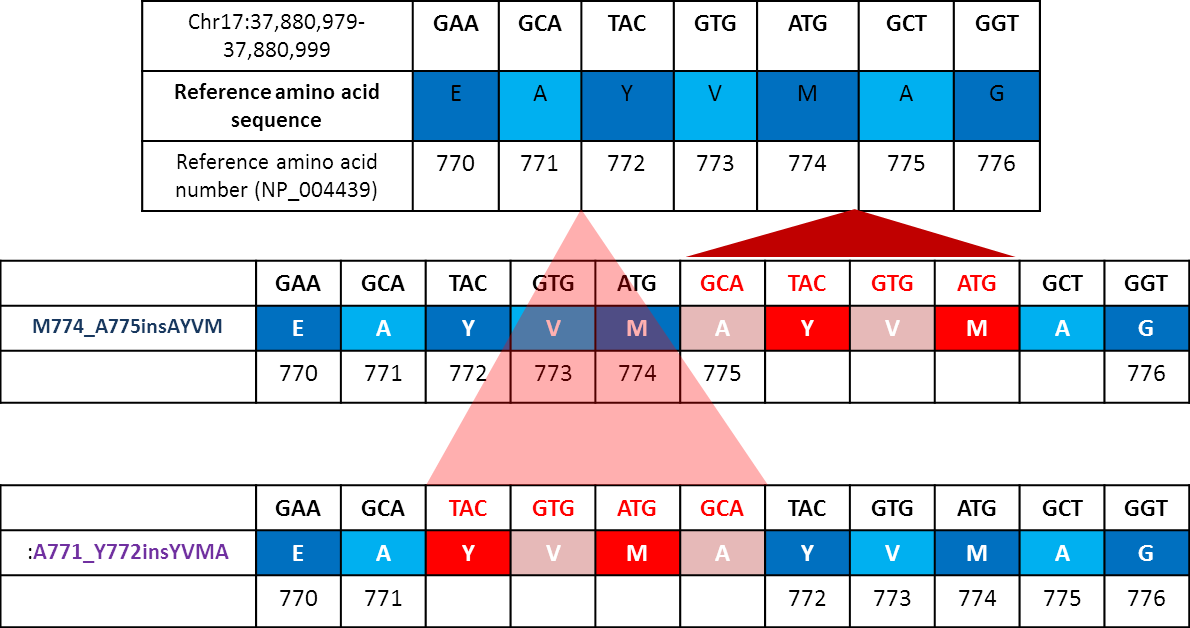
\includegraphics{assets/img/insertion_2.png}

\end{frame}

\begin{frame}{Nature volume 554, pages 189--194 (08 February
2018)\textsuperscript{2}}
\protect\hypertarget{nature-volume-554-pages-189194-08-february-2018--hyman_2018_her_nature}{}

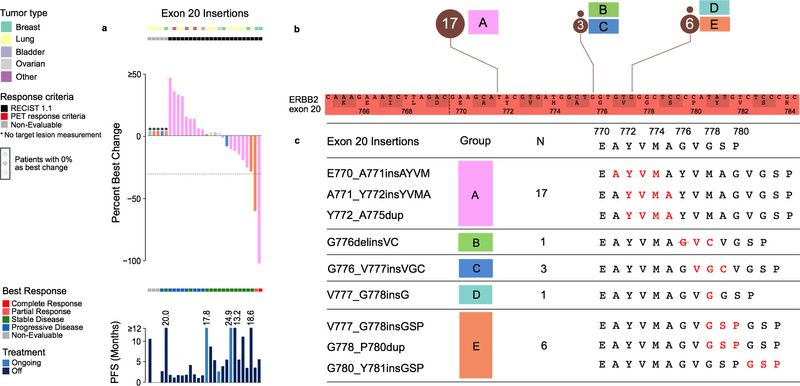
\includegraphics{assets/img/nature25475-sf4.jpg}

\end{frame}

\begin{frame}{Nat Med. 2018 May;24(5):638-646\textsuperscript{3}}
\protect\hypertarget{nat-med.-2018-may245638-646--robichaux_2018_mechanisms_natmed}{}

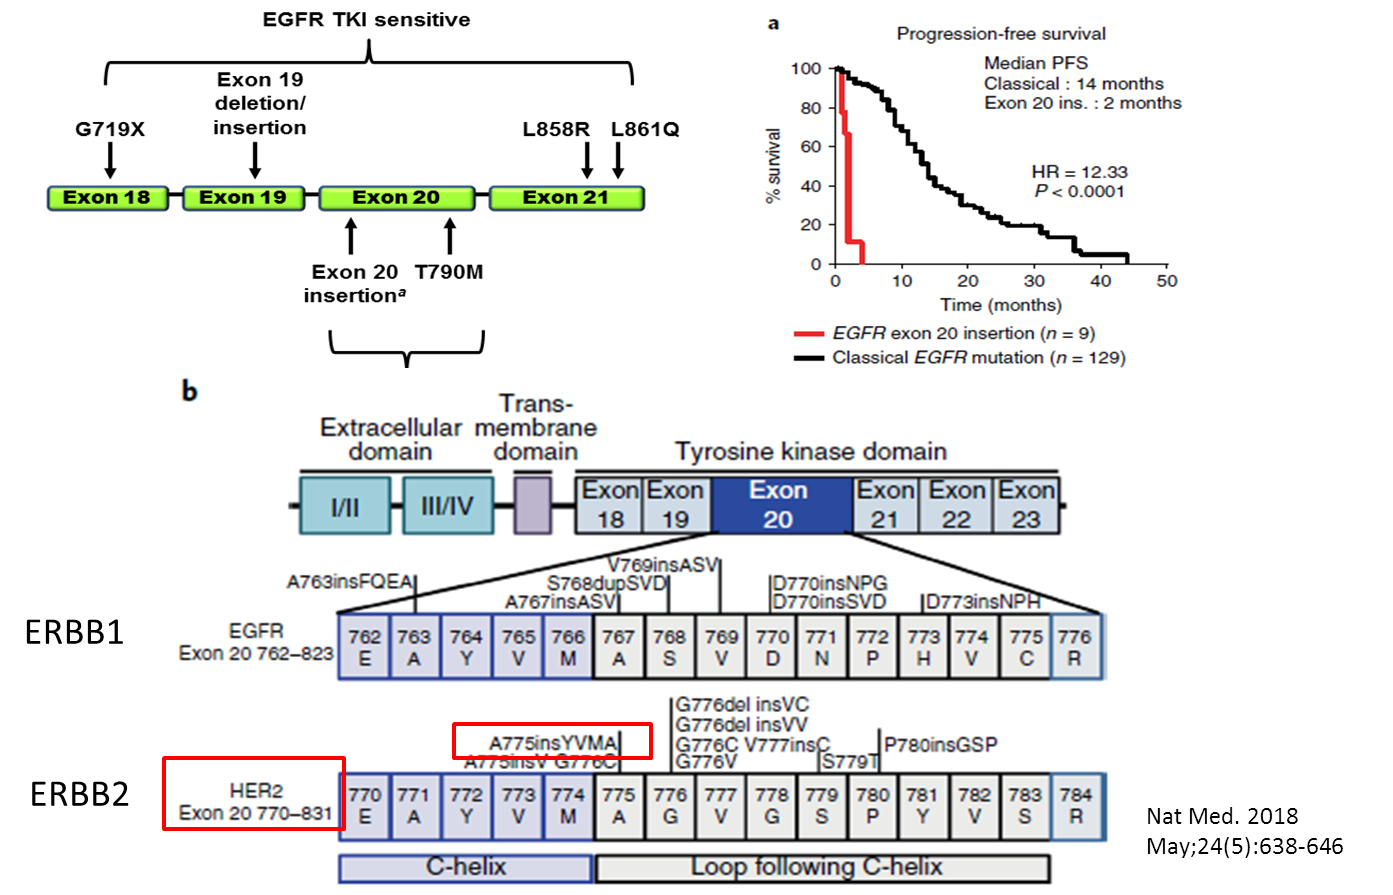
\includegraphics[width=\textwidth,height=2.08333in]{assets/img/TKI_resistance.png}

\end{frame}

\begin{frame}{Case 2}
\protect\hypertarget{case-2}{}

\begin{itemize}
\tightlist
\item
  F/80
\item
  Adenocarcinoma of lung
\end{itemize}

\end{frame}

\begin{frame}

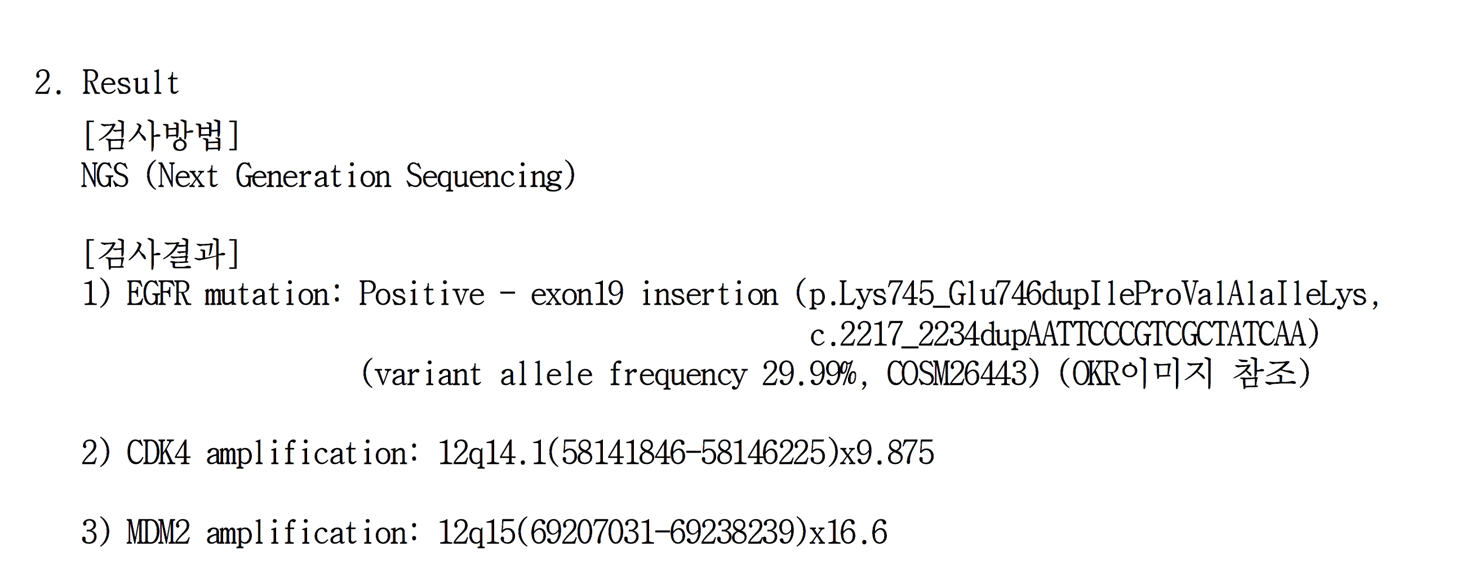
\includegraphics{assets/img/EGFR.png}

\end{frame}

\begin{frame}{EGFR Exon 19 insertion}
\protect\hypertarget{egfr-exon-19-insertion}{}

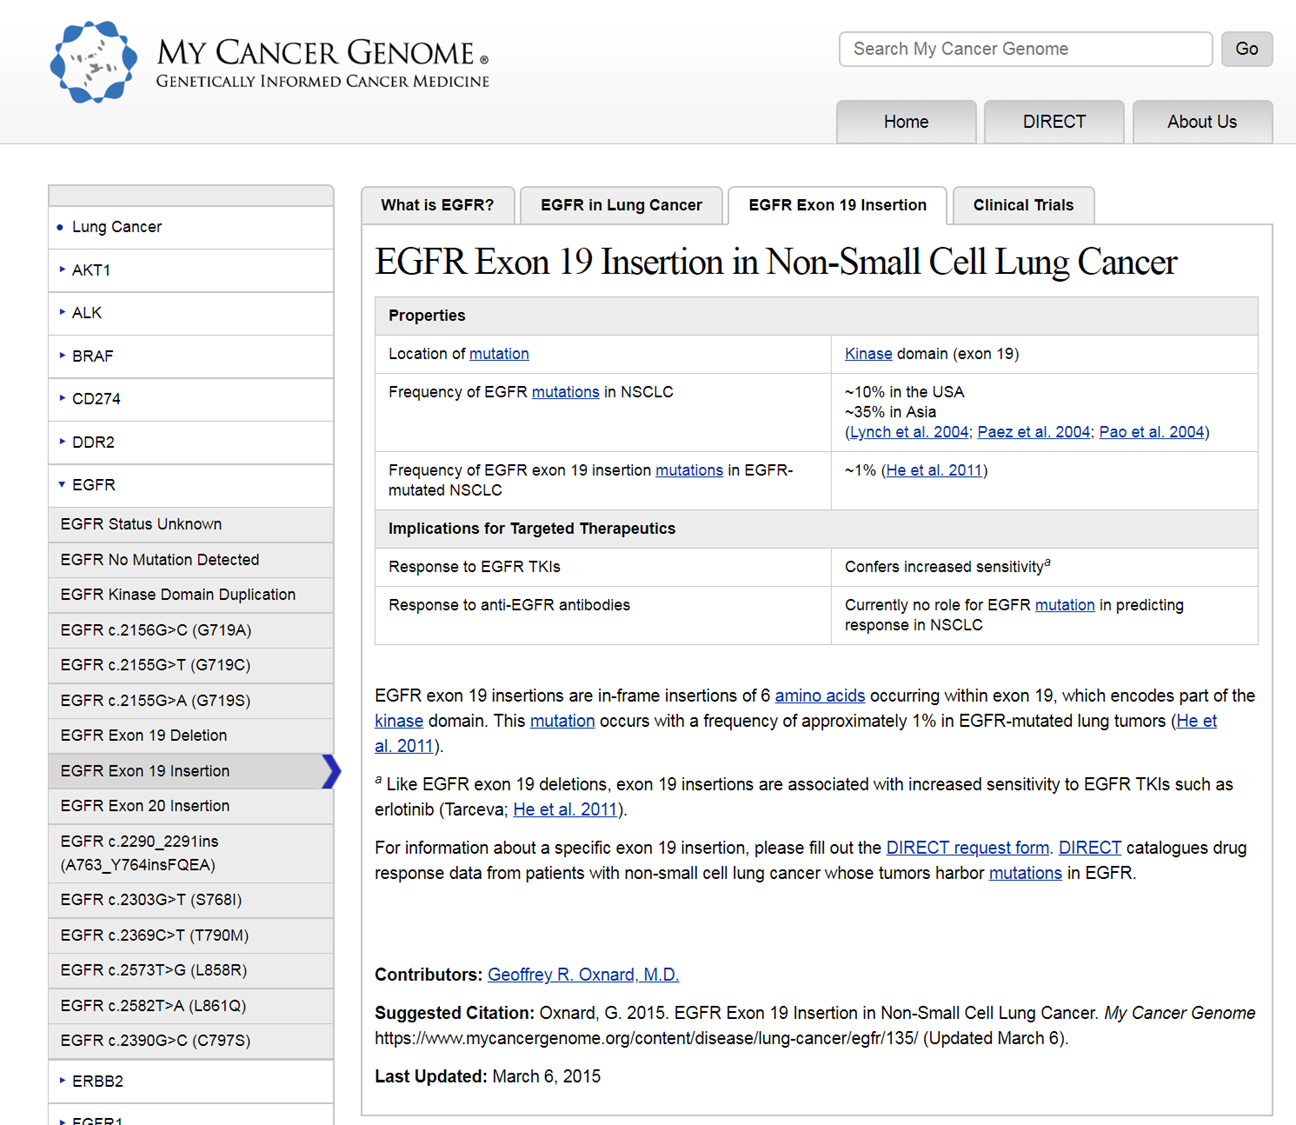
\includegraphics[width=\textwidth,height=7.29167in]{assets/img/mycancergenome.png}

\end{frame}

\begin{frame}{Annotation Redundancy EGFR exon 19 insertion}
\protect\hypertarget{annotation-redundancy-egfr-exon-19-insertion}{}

\begingroup\fontsize{8}{10}\selectfont

\begin{tabu} to \linewidth {>{\raggedright}X>{\raggedright}X>{\raggedright}X}
\hline
  & CDS mutation & AA mutation\\
\hline
Ion Reporter (IR) & c.2234\_2235ins & p.V738\_K739insKIPVAI\\
\hline
Cosmic & c.2232\_2233ins & p.K745\_E746insIPVAIK\\
\hline
Pathology  Report & c.2217\_2234dup & p.K745\_E750dupIPVAIK\\
\hline
Clinical Cancer Reserch & c.2217\_2234dup & p.K745\_E746insIPVAIK\\
\hline
\end{tabu}
\endgroup{}

\end{frame}

\begin{frame}{Allignment}
\protect\hypertarget{allignment}{}

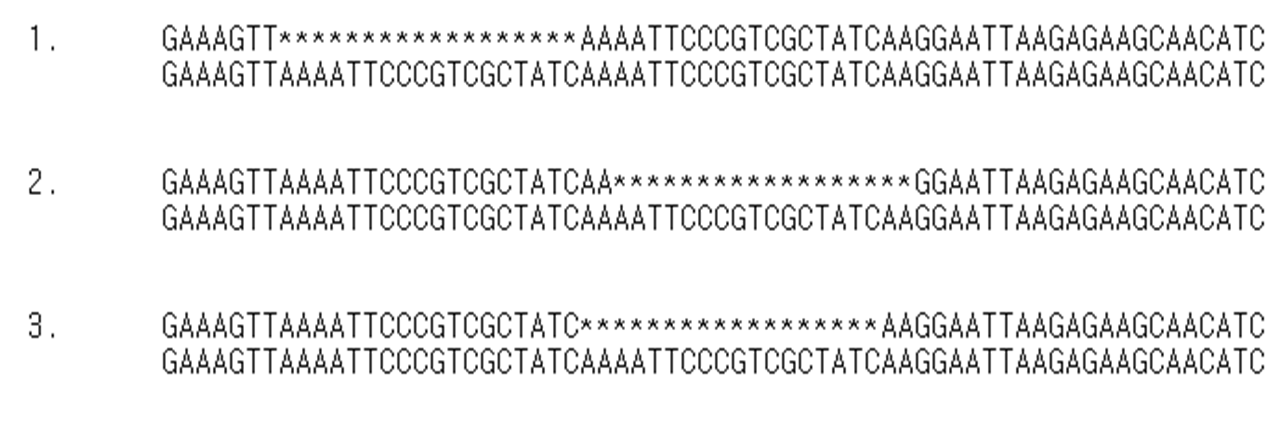
\includegraphics{assets/img/sequence.png}

\end{frame}

\begin{frame}{Clin Cancer Res; 18(6); 1790--7\textsuperscript{4}}
\protect\hypertarget{clin-cancer-res-186-17907--he_2012_egfr_clinicalcancerresearch}{}

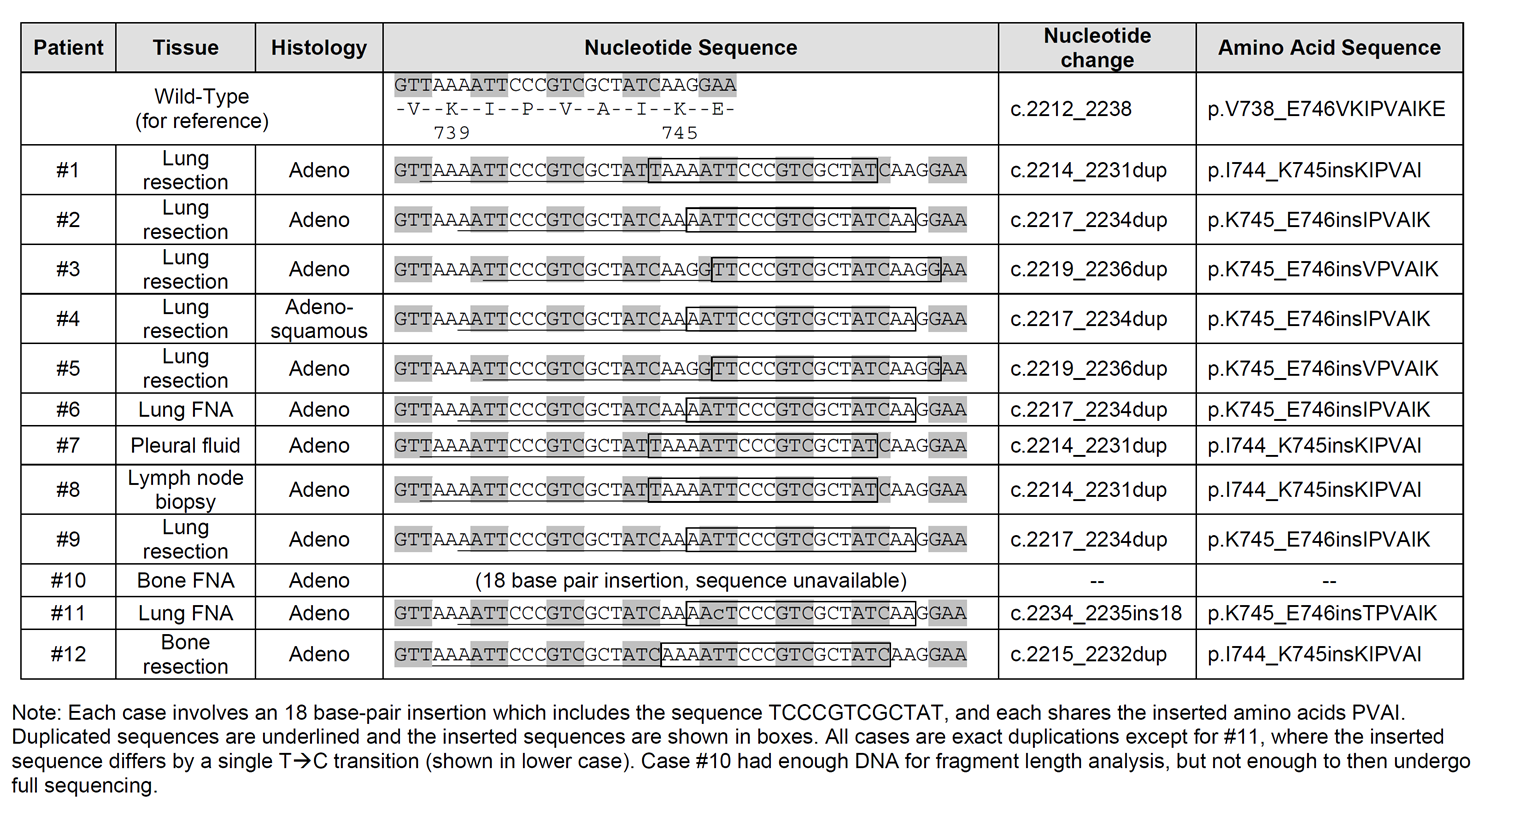
\includegraphics{assets/img/exon19.png}

\end{frame}

\begin{frame}{Mutation Nomenclature\textsuperscript{5}}
\protect\hypertarget{mutation-nomenclature--dunnen_2000_mutation_hummutat}{}

\begin{quote}
No recommendations have been made to describe duplications. Although
they can be seen as a specific type of insertion, and could be described
as such, they often originate through other mutational mechanisms. We
therefore prefer to provide a distinctive designation of this type of
sequence change
\end{quote}

\end{frame}

\begin{frame}{HGVS vs VEP}
\protect\hypertarget{hgvs-vs-vep}{}

\begin{itemize}
\tightlist
\item
  HGVS Recommendations for the Description of Sequence\\
\item
  Variants: 2016 Update
\end{itemize}

\begin{block}{The Ensembl Variant Effect Predictor}

\end{block}

\end{frame}

\begin{frame}{HGVS Recommendations for the Description of Sequence
Variants: 2016 Update}
\protect\hypertarget{hgvs-recommendations-for-the-description-of-sequence-variants-2016-update}{}

\begin{block}{\url{http://varnomen.hgvs.org/recommendations/}}

\end{block}

\end{frame}

\begin{frame}{Conclusions}
\protect\hypertarget{conclusions}{}

\begin{itemize}
\tightlist
\item
  Redundant annotation

  \begin{itemize}
  \tightlist
  \item
    ERBB2 exon20, EGFR exon19 insertion/duplication
  \end{itemize}
\end{itemize}

\end{frame}

\begin{frame}[allowframebreaks]{References}
\protect\hypertarget{references}{}

\hypertarget{refs}{}
\leavevmode\hypertarget{ref-__what_}{}%
1. What is the Variant Effect Predictor (VEP)? \textbar{} Ensembl
Genomes.

\leavevmode\hypertarget{ref-hyman_2018_her_nature}{}%
2. Hyman, D.M., Piha-Paul, S.A., Won, H., Rodon, J., Saura, C., Shapiro,
G.I., Juric, D., Quinn, D.I., Moreno, V., Doger, B., et al. (2018). HER
kinase inhibition in patients with HER2- and HER3-mutant cancers. Nature
\emph{554}, 189--194.

\leavevmode\hypertarget{ref-robichaux_2018_mechanisms_natmed}{}%
3. Robichaux, J.P., Elamin, Y.Y., Tan, Z., Carter, B.W., Zhang, S., Liu,
S., Li, S., Chen, T., Poteete, A., Estrada-Bernal, A., et al. (2018).
Mechanisms and clinical activity of an EGFR and HER2 exon 20--selective
kinase inhibitor in non--small cell lung cancer. Nature Medicine
\emph{24}, 638.

\leavevmode\hypertarget{ref-he_2012_egfr_clinicalcancerresearch}{}%
4. He, M., Capelletti, M., Nafa, K., Yun, C.-H., Arcila, M.E., Miller,
V.A., Ginsberg, M.S., Zhao, B., Kris, M.G., Eck, M.J., et al. (2012).
EGFR Exon 19 Insertions: A New Family of Sensitizing EGFR Mutations in
Lung Adenocarcinoma. Clinical Cancer Research \emph{18}, 1790--1797.

\leavevmode\hypertarget{ref-dunnen_2000_mutation_hummutat}{}%
5. Dunnen, J.T. den, and Antonarakis, S.E. (2000). Mutation nomenclature
extensions and suggestions to describe complex mutations: A discussion.
Human Mutation \emph{15}, 7--12.

\end{frame}

\end{document}
